\chapter{プリバーナ方式液体酸素気化実験}
\newcommand{\FigAddThree}{./src/Chapter3/Figure}
\section{可視化実験}
\subsection{実験目的、設定条件}
本実験ではO/F=50以上での酸素とPMMAの反応となるため、燃焼器内部の状態を確認した。
燃焼器外殻が透明な供試体を使用し、高速度カメラによる燃焼室内部の可視化を目的とした実験を行った。
液体酸素流量が$0.02kg/s$程度になるようにHe圧力を設定し、燃料グレインは$15mm,30mm$の2種類を使用し試験を行った。
本実験は表\ref{S1TestCondition}の設定条件で行った。

\subsection{実験結果および考察}
5回の燃焼器か試験を実施した。
No.1の燃焼気化中の計測データを時間履歴を図\ref{fig:S1Case1}に示す。
インジェクタ上流の酸素温度は、沸点異常であり、LOXの安定供給はできなかった。
ノズル上流及び下流の温度は、K熱電対の測定可能上限1280℃を超えており、実験後に熱電対を確認した所、焼損していることがわかった。
プリバーナ部のベークライトスペーサ及びベークライトのバッフルプレートは焼損しており、酸素の加熱に寄与したことがわかる。
バッフルプレートはインジェクタ直下が激しく焼損しており、酸素がいき良いよく衝突していることがわかった。
\\
No.5の燃焼気化中の計測データの時間履歴を図\ref{fig:S1Case5}に示す。
インジェクタ上流の酸素温度は、沸点以下に下がっており、LOXを安定に供給はできた。
タービン流量計は不具合のため計測できていないが、オリフィスもしくはインジェクタの差圧から流量を見積もった結果から、
実験後半では比較的一様にLOXを供給できていることがわかる。
図\ref{fig:S1AfBaffle}に実験後のバッフルプレートの様子を示す。
焼損が激しく孔同士が繋がったことがわかる。
\\
燃焼気化試験結果のまとめを表\ref{tab:S1Result}に示す。
また、燃料グレインおよびスペーサ、バッフルプレート、グラファイトノズルの質量の変化のまとめを表\ref{tab:S1DifSBN}に示す。
No.1~3の実験では、インジェクタ上流の酸素温度は沸点以上で、安定的にLOXを供給できなかった。
No.4および5では、実験後半で沸点以下に下がっており、LOXを供給することができた。
LOX流量はタービン流量計による計測ができていない。
今回はインジェクタ上下流差圧を用いてデータを整理した。
O/Fは、目標の50からは大きく外れている。
\\
グラファイトノズルは全く焼損していないが、ベークライトのスペーサとバッフルプレートは焼損が激しかった。
そのため、大きな流量および長時間での実験が実施できなかった。
\\
No.5試験では、燃焼の様子の高速度カメラでの撮影に成功した。
図\ref{fig:InsideofChamber}にNo.5の燃焼の様子を示す。
白く発光しているところが火炎が存在する領域であるが、
インジェクター直下及びバッフルプレート直上にて激しく発光しているため、
火炎が滞留していることが確認できる。
また実験映像よりプリバーナ部分での逆流が確認でき、
プリバーナ部で激しく混合していることがわかった。

\input{./src/Chapter3/S1Conclusion}


\section{実証機モデルの性能計算}
実験によって得られた計測データを元に実証機モデルの性能計算を評価し、
実証器モデルの寸法を決定した。
性能計算は以下の要領で計算を行った。
\begin{itemize}
\item 酸化剤質量流束より燃料流量を推定
\item 燃焼室圧力、O/FよりnasaCEAで化学平衡計算
\item 計算結果より平均燃料グレイン形状を推定
\item 燃焼終了時間まで繰り返す
\end{itemize}
酸化剤質量流束は燃焼室に噴射する酸化剤質量流量と燃料ポート断面積から求めた。
検討しているハイブリッドロケットエンジンの酸化剤質量流量は最大$10[kg/s]$を想定しているため(\ref{})、
本検討でも酸化剤質量流量は$10[kg/s]$とした。

実証機の設計諸元\ref{tab:RealModel}と寸法及び概略図を表と図に示す。

\section{水流し試験}
本実験では流量計測にタービン流量計の他にオリフィス差圧とインジェクタ差圧を使用した。
差圧から流量を計測するために、各差圧の流量係数を確認する必要がある。
GHe供給圧をパラメータとし、水を30秒以上流し、噴出した水の総量から、水の流量を求めた。水の噴射の様子を図に示す。
\\
流量定数はベルヌーイの定理と連続の式から導出できる。
\begin{eqnarray}
P_{1} + \frac{1}{2} \rho_{1} u^2_{1} &=& P_{2} + \frac{1}{2} \rho_{2} u^2_{2}  \nonumber \\
u^2_{2} - u^2_{1} &=& \frac{2(P_{1}-P_{2})}{\rho} 
\label{eq:vel}
\end{eqnarray}
\begin{eqnarray}
u_{1}A_{1} &=& u_{2}A_{2}  \nonumber \\
u_{2} &=& u_{1}\frac{A_{1}}{A_{2}}
\label{eq:con}
\end{eqnarray}
\ref{eq:con}を\ref{eq:vel}に代入する。
\begin{eqnarray}
u_{2}=\frac{1}{\sqrt{1-(\frac{A_{2}}{A_{1}})^2}}\sqrt{\frac{2(P_{1}-P_{2})}{\rho}}
\label{eq:Velocity}
\end{eqnarray}
流量は$Q=u_{2}A_{2}$であるので、
\begin{eqnarray}
Q=u_{2}A_{2}=\frac{A_{2}}{\sqrt{1-(\frac{A_{2}}{A_{1}})^2}}\sqrt{\frac{2(P_{1}-P_{2})}{\rho}}
\label{eq:VFlux}
\end{eqnarray}
となり流量が求まる。ここで$CA=\frac{A_{2}}{\sqrt{1-(\frac{A_{2}}{A_{1}})^2}}$とすると、
\begin{eqnarray}
Q=CA\sqrt{\frac{2(P_{1}-P_{2})}{\rho}}
\label{eq:IdealFlux}
\end{eqnarray}
となる。$C$は流量係数で、$C=\frac{流量実測値}{流量計算値}$で求まる。$A$はオリフィス断面積である。
オリフィス断面積は$2.01 \times 10^{-6}mm$,インジェクタ断面積は$1.41 \times 10^{-6}mm$である。
本試験結果を表\ref{tab:Water}に示す。
\\
本試験でのインジェクタ及びオリフィスでの流量係数はそれぞれ$0.52$と$1.06$となった。
インジェクタの流量係数が設計時の想定流量係数$0.7$より小さくなった。
これはインジェクタ上流のマニホールド部の体積が小さく、流れの整流が十分ではなく、インジェクタ孔へ流れる流体の抵抗が大きくなったことが原因として考えられる。
\\
オリフィス流量係数は、$1$を超えている。計算上のオリフィス内径は$1.6mm$を用いているが、実際使用したものは$1.6mm$以上あるからと思われる。
\\
この試験により、実験上問題となる以上はないことが確認できた。

\begin{table}[htb]
\begin{center}
\caption{水流し試験結果}
\scriptsize
%\begin{tabular*}{200mm}{@{\extracolsep{\fill}}|c|c|c|c|c|c|c|c|c|c|} \hline
\begin{tabular}{|c|c|c|c|c|c|c|c|c|c|} \hline
No. & \shortstack{設定He\\圧力} & \shortstack{インジェクタ\\上流圧} & 流量 & \shortstack{インジェクタ\\差圧} & \shortstack{インジェクタ\\流量} & \shortstack{インジェクタ\\流量係数} & \shortstack{オリフィス\\差圧} & \shortstack{オリフィス\\理論流量} & \shortstack{オリフィス\\流量係数} \\ \cline{2-10}
 & MPaA & MPaA & L/s & MPa & L/s & - & MPa & L/s & - \\ \hline
1 & 0.6 & 0.55 & 0.021 & 0.45 & 0.042 & 0.51 & 0.058 & 0.022 & 0.99 \\ \hline
2 & 1.09 & 0.94 & 0.030 & 0.84 & 0.058 & 0.52 & 0.102 & 0.029 & 1.05 \\ \hline
3 & 1.61 & 1.40 & 0.037 & 1.30 & 0.072 & 0.51 & 0.149 & 0.035 & 1.06 \\ \hline
4 & 2.12 & 1.82 & 0.043 & 1.72 & 0.083 & 0.52 & 0.200 & 0.040 & 1.06 \\ \hline
5 & 3.10 & 2.68 & 0.053 & 2.58 & 0.102 & 0.52 & 0.300 & 0.049 & 1.07 \\ \hline
\end{tabular}
\label{tab:Water}
\end{center}
\end{table}



\begin{table}[htb]
\begin{center}
\caption{可視化実験設定条件}
\small
\begin{tabular}{|c|c|c|c|c|c|} \hline
No. & 設定He圧力 & 燃焼時間 & \multicolumn{3}{|c|}{グレイン(PMMA)} \\ \cline{2-6}
 & MPaA & s & 長さ[mm] & 外径[mm] & 内径[mm]  \\ \hline
1 & 1.2 & 3 & & & \\ \cline{1-3}
2 & 1.2 & 3 & 15 & & \\ \cline{1-3}
3 & 2.0 & 5 & & 50 & 30  \\ \cline{1-4}
4 & 1.2 & 5 &30  &  & \\ \cline{1-3}
5 & 1.2 & 4 &  &  &  \\ \hline
\end{tabular}
\label{tab:S1TestCondition}
\end{center}
\end{table}

\begin{table}[htb]
\begin{center}
\caption{設定条件}
\small
\begin{tabular}{|c|c|c|c|c|c|} \hline
No. & 設定He圧力 & 燃焼時間 & \multicolumn{3}{|c|}{グレイン(PMMA)} \\ \cline{2-6}
 & MPaA & s & 長さ[mm] & 外径[mm] & 内径[mm]  \\ \hline
1 & 3.4 & 5.0 & & & \\ \cline{1-3}
2 & 4.9 & 8.0 &7.5 & & \\ \cline{1-3}
3 & 3.6 & 8.0 & & & \\ \cline{1-4}
4 & 3.1 & 5.0 & & & \\ \cline{1-4}
5 & 5.0 & 6.5 & & 50 & 30 \\ \cline{1-4}
6 & 4.3 & 6.5 & 15 & &  \\ \cline{1-4}
7 & 4.0 & 6.5 & & &  \\ \cline{1-4}
8 & 3.3 & 6.5 & & &  \\ \hline
\end{tabular}
\label{tab:S2TestCondition}
\end{center}
\end{table}

\begin{figure}
\centering
\caption{実験結果}
\includegraphics[width=10cm]{\FigAddThree/png/S1Result.png}
\label{tab:S1Result}
\end{figure}

\begin{figure}
\centering
\caption{各部材の質量変化量}
\includegraphics[width=10cm]{\FigAddThree/png/S1DifSBN.png}
\label{tab:S1DifSBN}
\end{figure}

\begin{table}[htb]
\begin{center}
\caption{燃料後退速度係数}
\small
\begin{tabular}{|c|c|c|} \hline
				& A		& n		\\ \hline
7.5mm(Ave) 	& 0.0077	& 0.9487	\\ \hline
15mm(Ave) 	& 0.1358	& 0.4161	\\ \hline
15mm(Mid) 	& 0.0456	& 0.4884	\\ \hline
15mm(Rear) 	& 0.2649	& 0.3701	\\ \hline
Refference 	& 0.0145	& 0.749 	\\ \hline
\end{tabular}
\label{tab:S3RegressionRate}
\end{center}
\end{table}

\begin{figure}
\centering
\includegraphics[width=11cm]{\FigAddThree/eps/Ex1.eps}
\caption{実験結果1}
\label{fig:S1Case1}
\end{figure}

\begin{figure}
\centering
\includegraphics[width=11cm]{\FigAddThree/eps/Ex2.eps}
\caption{実験結果5}
\label{fig:S1Case5}
\end{figure}

\begin{figure}
\centering
\includegraphics[width=10cm]{\FigAddThree/png/S1AfBaffle.png}
\caption{燃焼試験終了後のバッフルプレート}
\label{fig:S1AfBaffle}
\end{figure}

\begin{figure}
\centering
\includegraphics[width=10cm]{\FigAddThree/png/InsideofChamber.png}
\caption{燃焼室内部の様子及び燃料流の挙動}
\label{fig:InsideofChamber}
\end{figure}


\begin{figure}
\centering
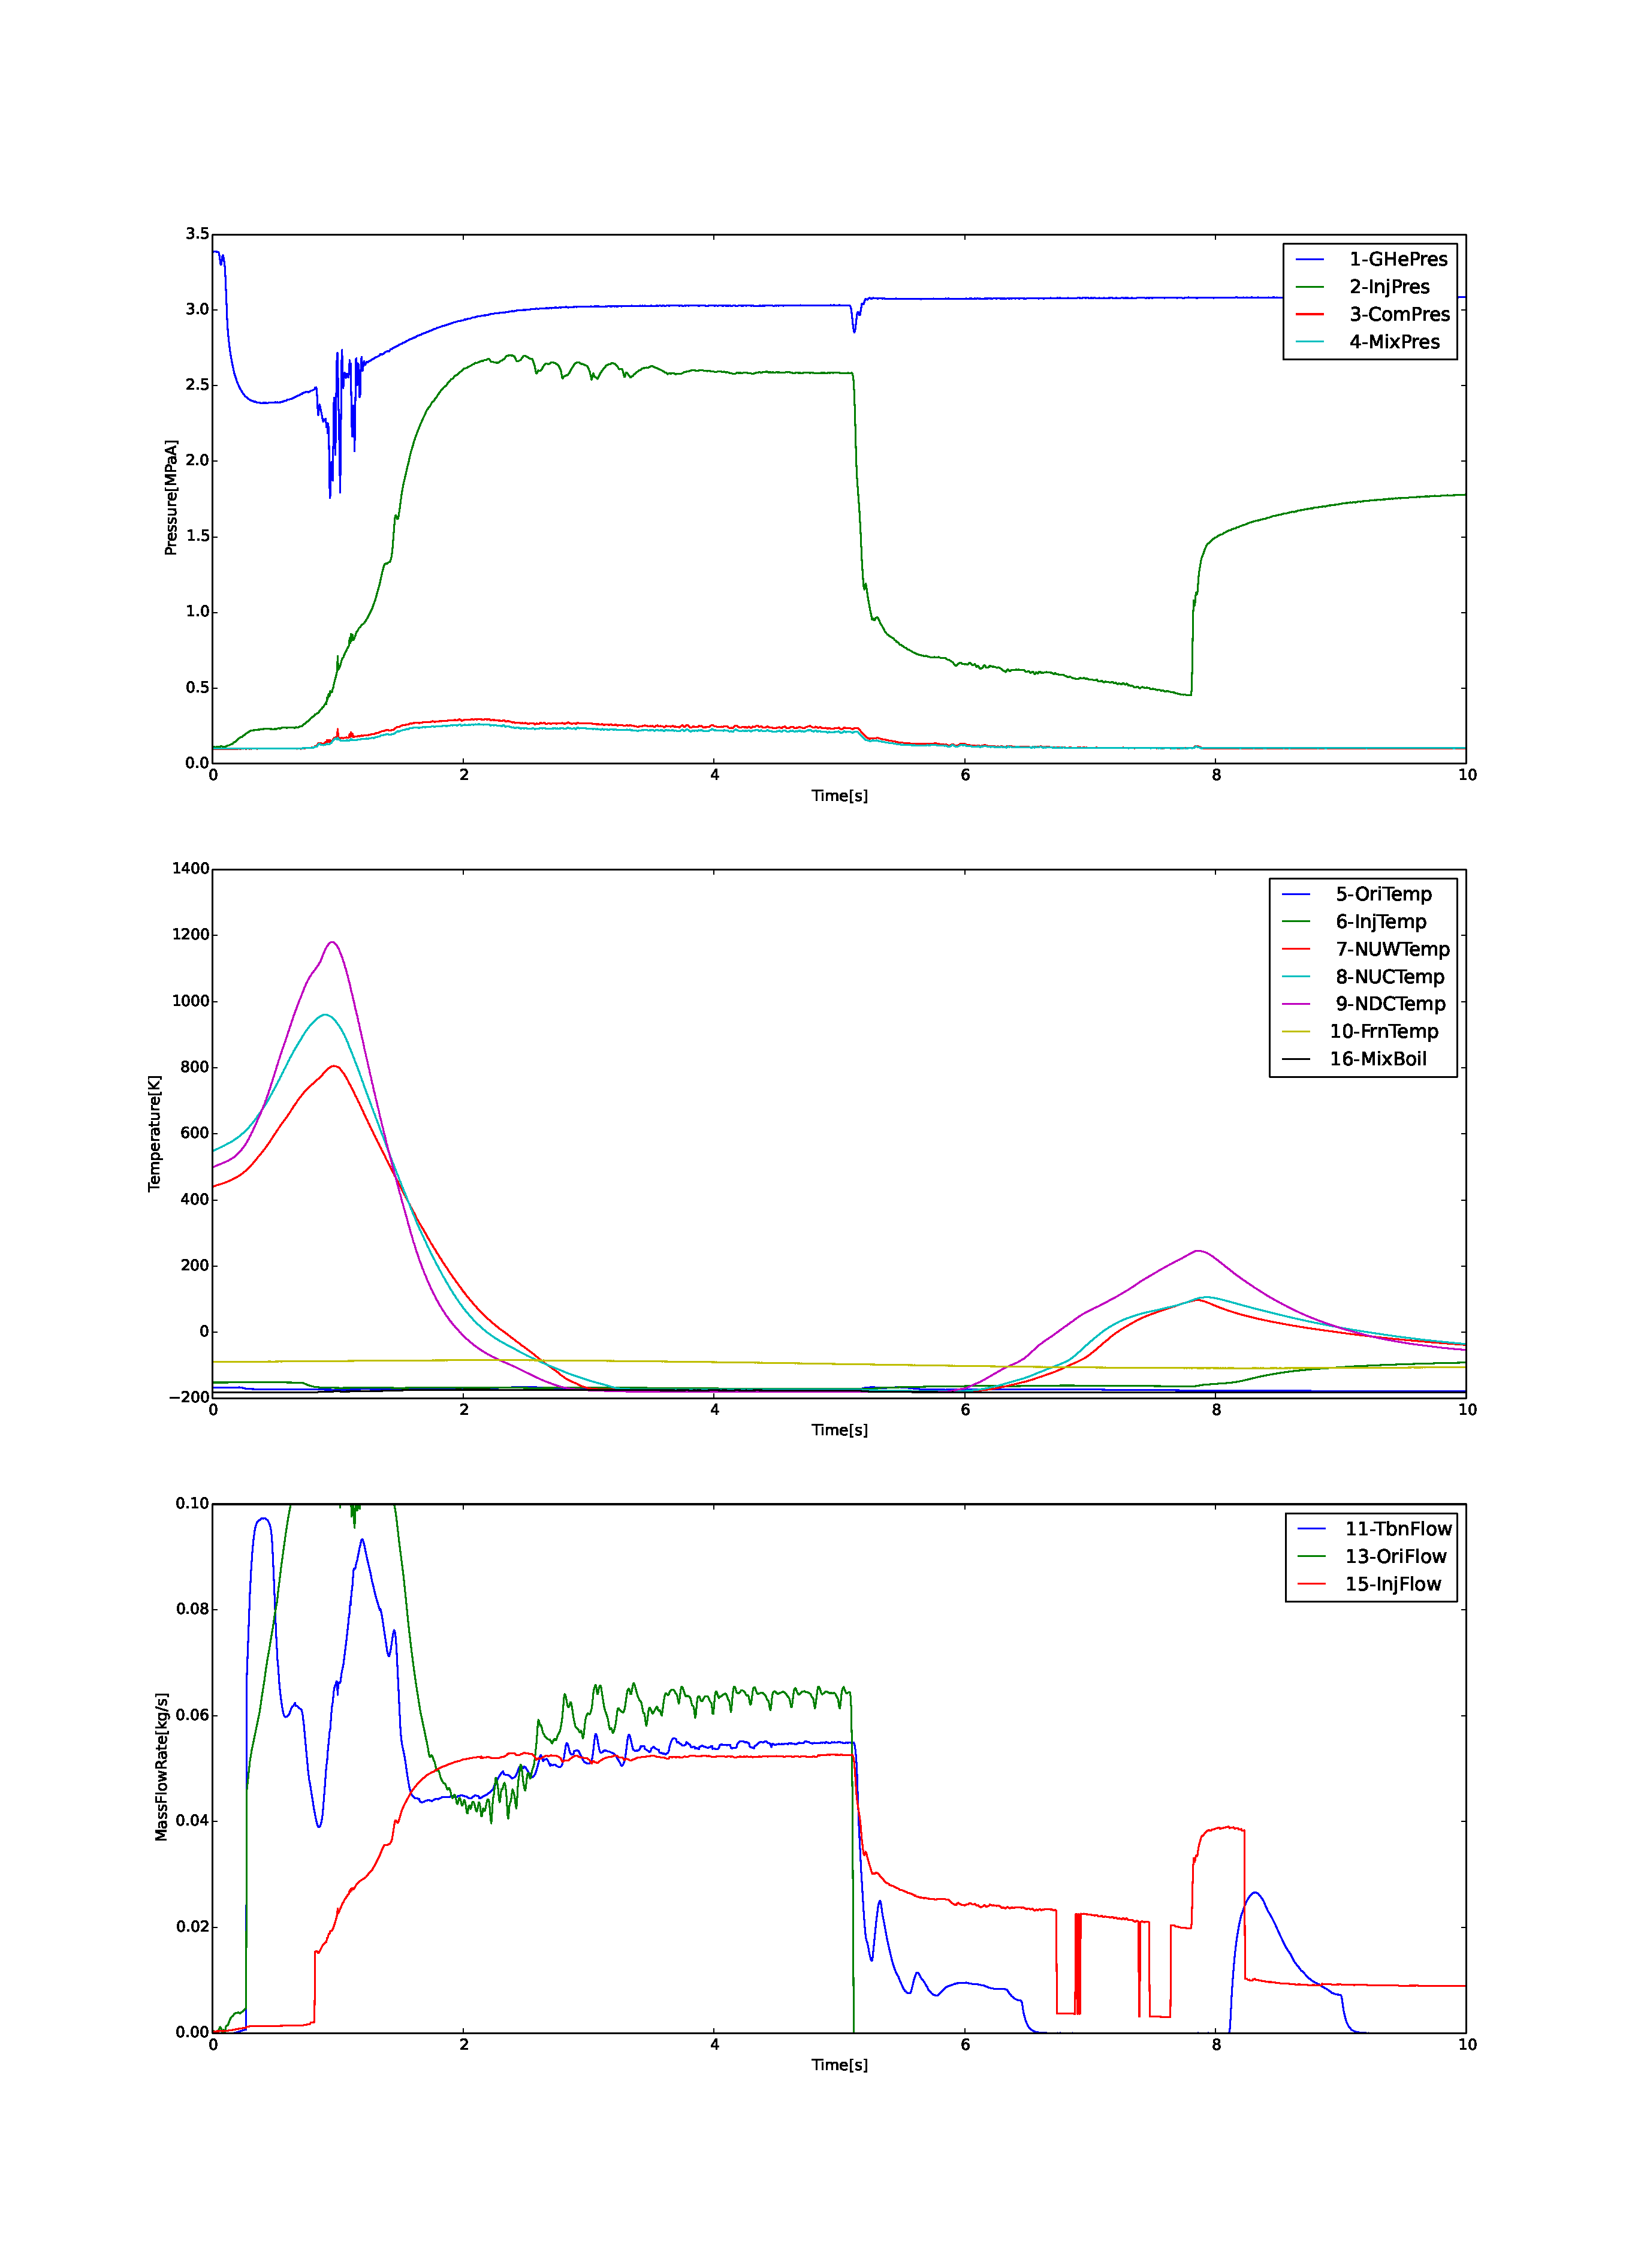
\includegraphics[width=11cm]{\FigAddThree/eps/Ex21.eps}
\caption{実験結果1}                                
\label{fig:S2Case1}                                
\end{figure}                                       

\begin{figure}                                     
\centering                                         
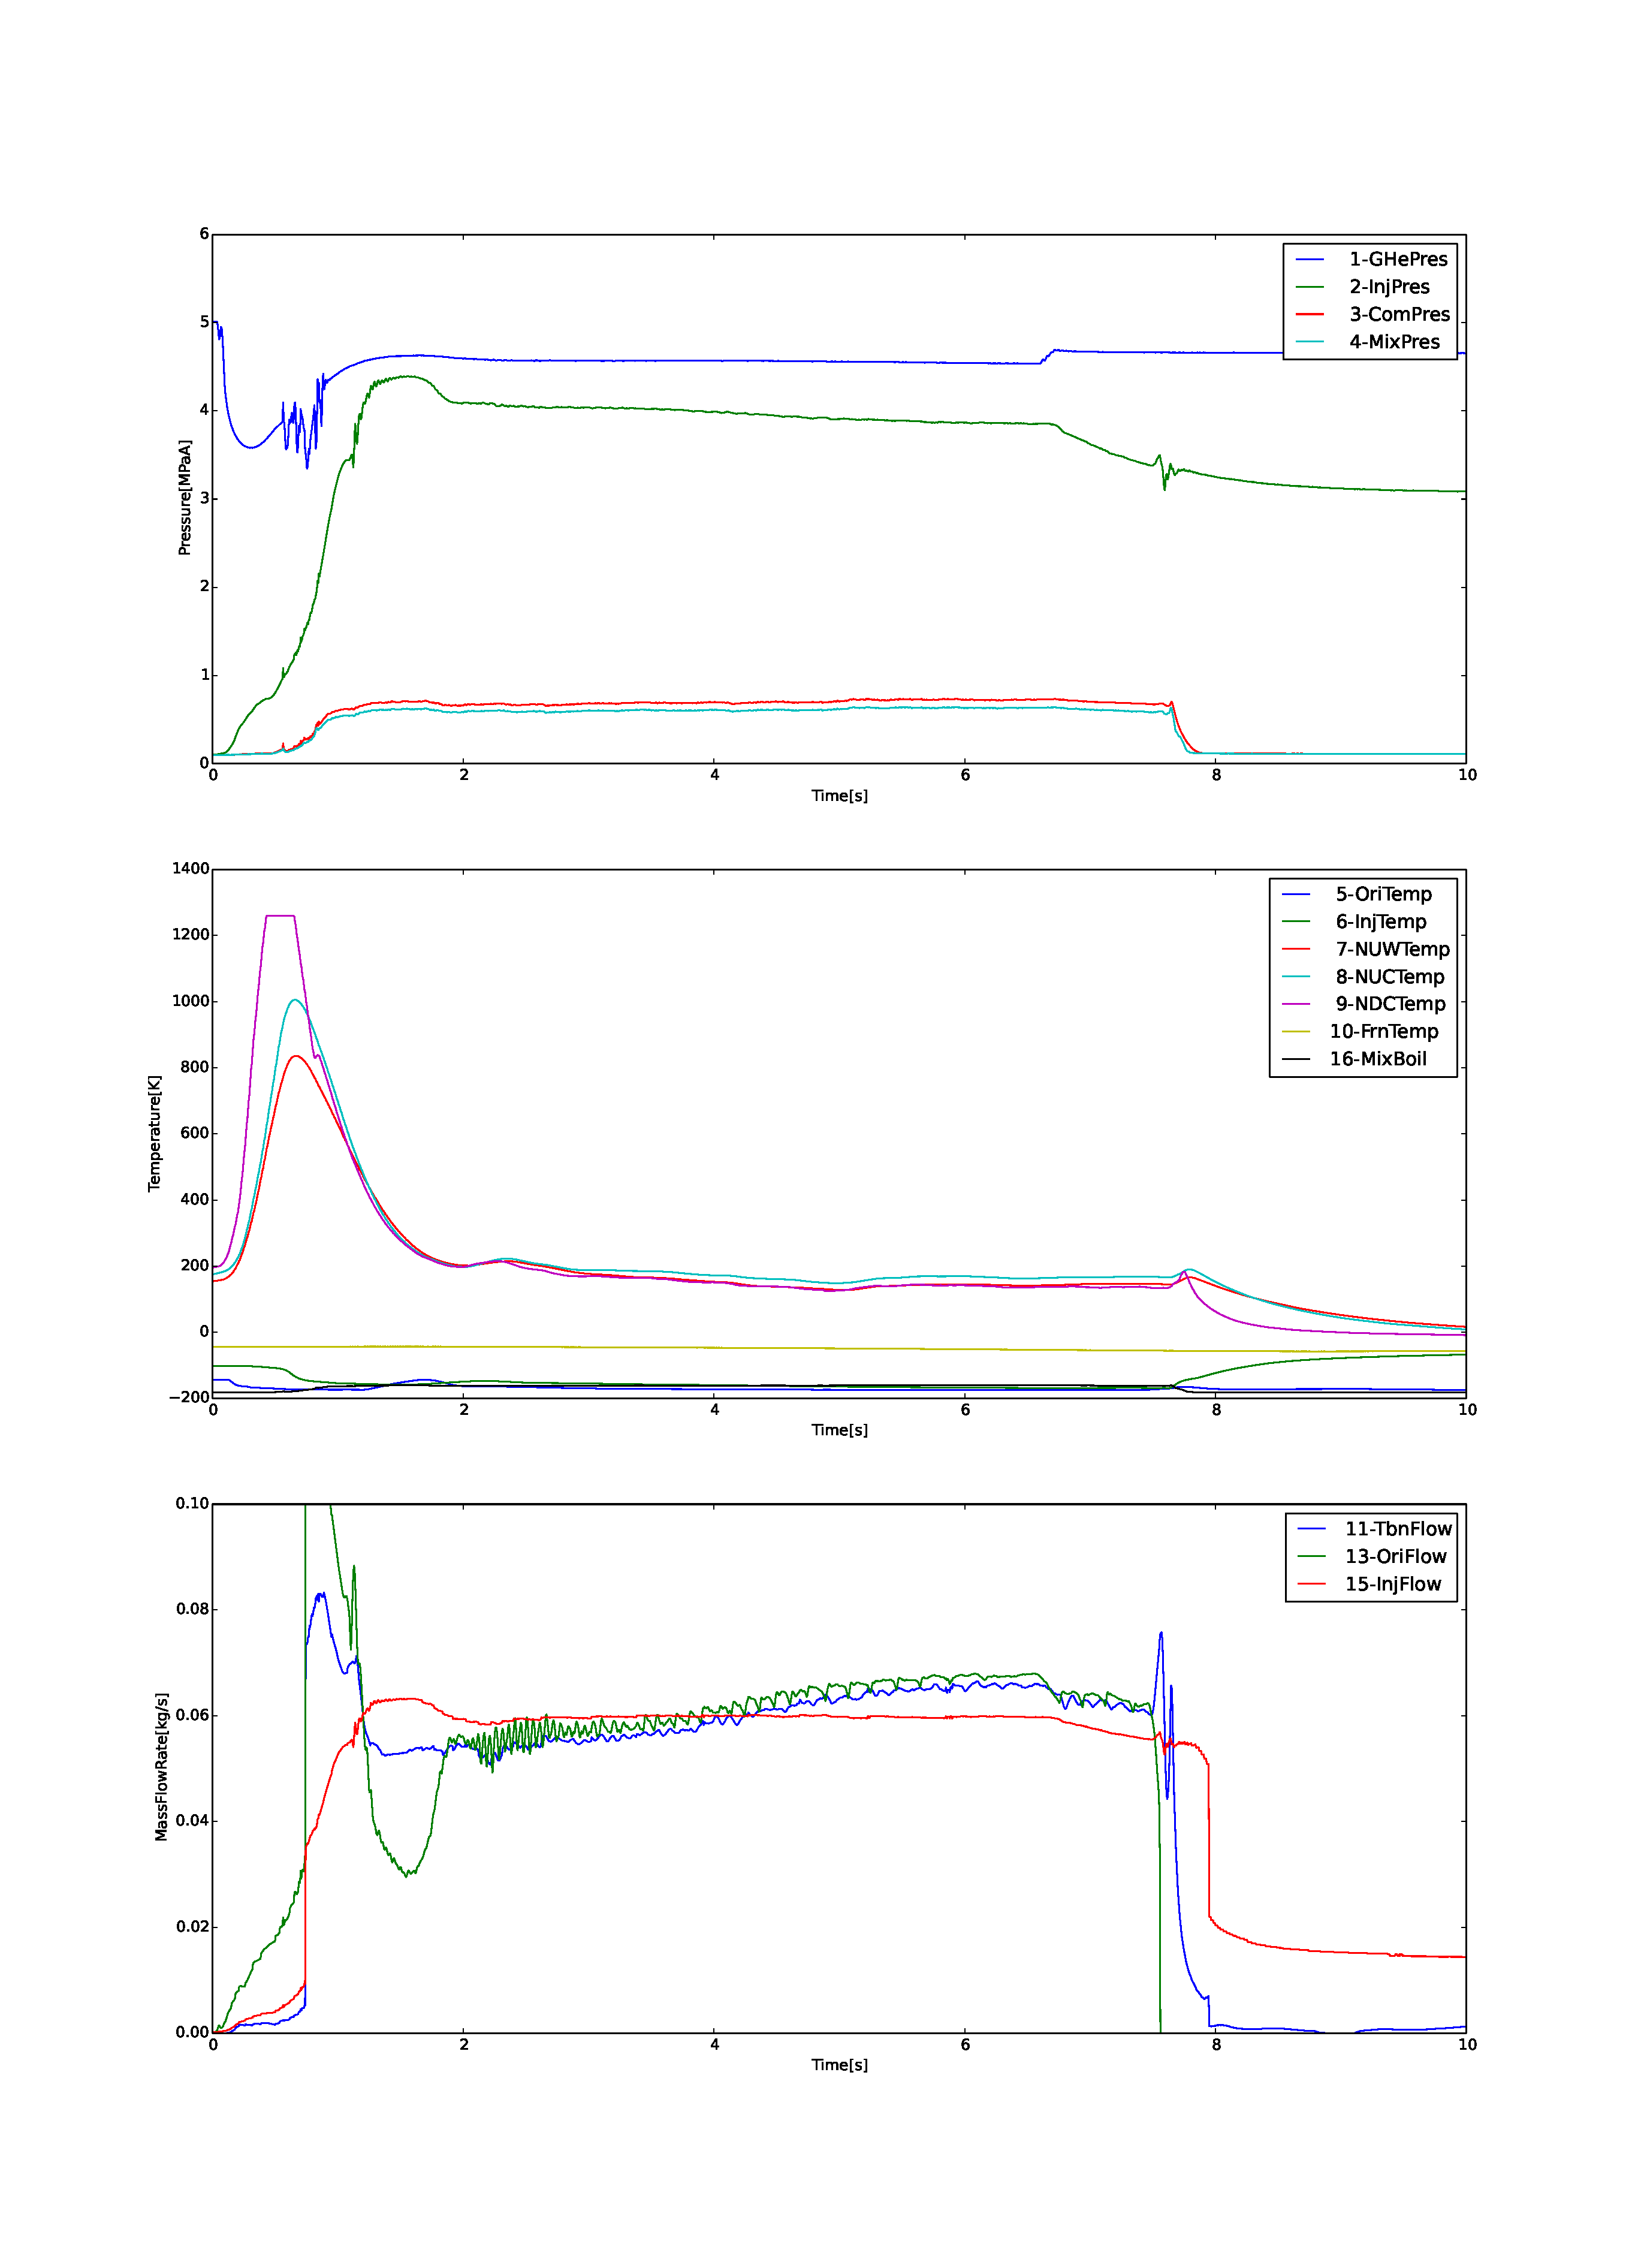
\includegraphics[width=11cm]{\FigAddThree/eps/Ex25.eps}
\caption{実験結果5}
\label{fig:S2Case5}
\end{figure}


\begin{figure}
\centering
\includegraphics[width=10cm]{\FigAddThree/png/rdotfit.png}
\caption{バッフルプレートを使用したLOX/PMMA燃料後退速度結果}
\label{fig:S3RegressionRate}
\end{figure}

\begin{figure}
\centering
\includegraphics[width=10cm]{\FigAddThree/png/AfGrain75.png}
\caption{燃焼試験終了後の$7.5mm$燃料グレイン}
\label{fig:S3Case1Grain}
\end{figure}

\begin{figure}
\centering
\includegraphics[width=10cm]{\FigAddThree/png/AfGrain15.png}
\caption{燃焼試験終了後の$15mm$燃料グレイン}
\label{fig:S3Case5Grain}
\end{figure}
